\documentclass{standalone}
\usepackage{tikz}

\begin{document}

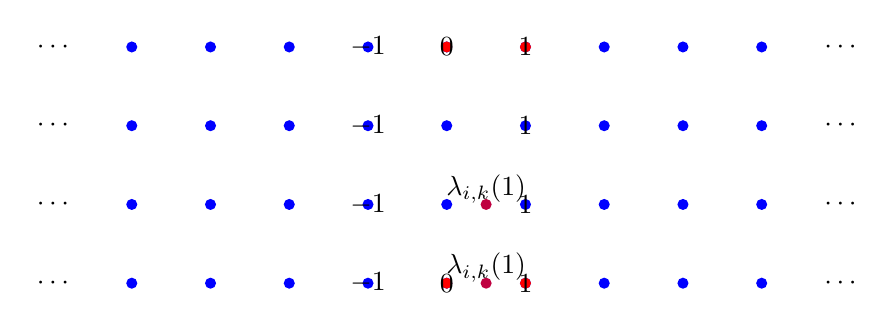
\begin{tikzpicture}
    % First row
    \foreach \x in {-4, -3, -2, -1, 0, 1, 2, 3, 4} {
        \fill[blue] (\x, 3) circle (2pt);
    }
    \foreach \x in {0, 1} {
        \fill[red] (\x, 3) circle (2pt);
    }
    \node at (-1, 3) {$-1$};
    \node at (0, 3) {$0$};
    \node at (1, 3) {$1$};

    % Second row
    \foreach \x in {-4, -3, -2, -1, 0, 1, 2, 3, 4} {
        \fill[blue] (\x, 2) circle (2pt);
    }
    \node at (-1, 2) {$-1$};
    \node at (1, 2) {$1$};

    % Third row
    \foreach \x in {-4, -3, -2, -1, 0, 1, 2, 3, 4} {
        \fill[blue] (\x, 1) circle (2pt);
    }
    \node at (-1, 1) {$-1$};
    \node at (1, 1) {$1$};
    \fill[purple] (0.5, 1) circle (2pt);
    \node at (0.5, 1.2) {$\lambda_{i,k}(1)$};

    % Fourth row
    \foreach \x in {-4, -3, -2, -1, 0, 1, 2, 3, 4} {
        \fill[blue] (\x, 0) circle (2pt);
    }
    \foreach \x in {0, 1} {
        \fill[red] (\x, 0) circle (2pt);
    }
    \node at (-1, 0) {$-1$};
    \node at (0, 0) {$0$};
    \node at (1, 0) {$1$};
    \fill[purple] (0.5, 0) circle (2pt);
    \node at (0.5, 0.2) {$\lambda_{i,k}(1)$};
    
    % Dots on the sides
    \node at (-5, 3) {$\cdots$};
    \node at (5, 3) {$\cdots$};
    \node at (-5, 2) {$\cdots$};
    \node at (5, 2) {$\cdots$};
    \node at (-5, 1) {$\cdots$};
    \node at (5, 1) {$\cdots$};
    \node at (-5, 0) {$\cdots$};
    \node at (5, 0) {$\cdots$};
\end{tikzpicture}

\end{document}